\documentclass{beamer}

\usepackage[tech]{sfocs-slides}

% \usepackage{tcolorbox}

\colorlet{structfgcolor}{white}

\date{\today}
\title{Elegant Coding in Elm}
\author{Long}

\begin{document}

\maketitle

\section{Introduction}

\begin{frame}{Discussion on Code Quality}
	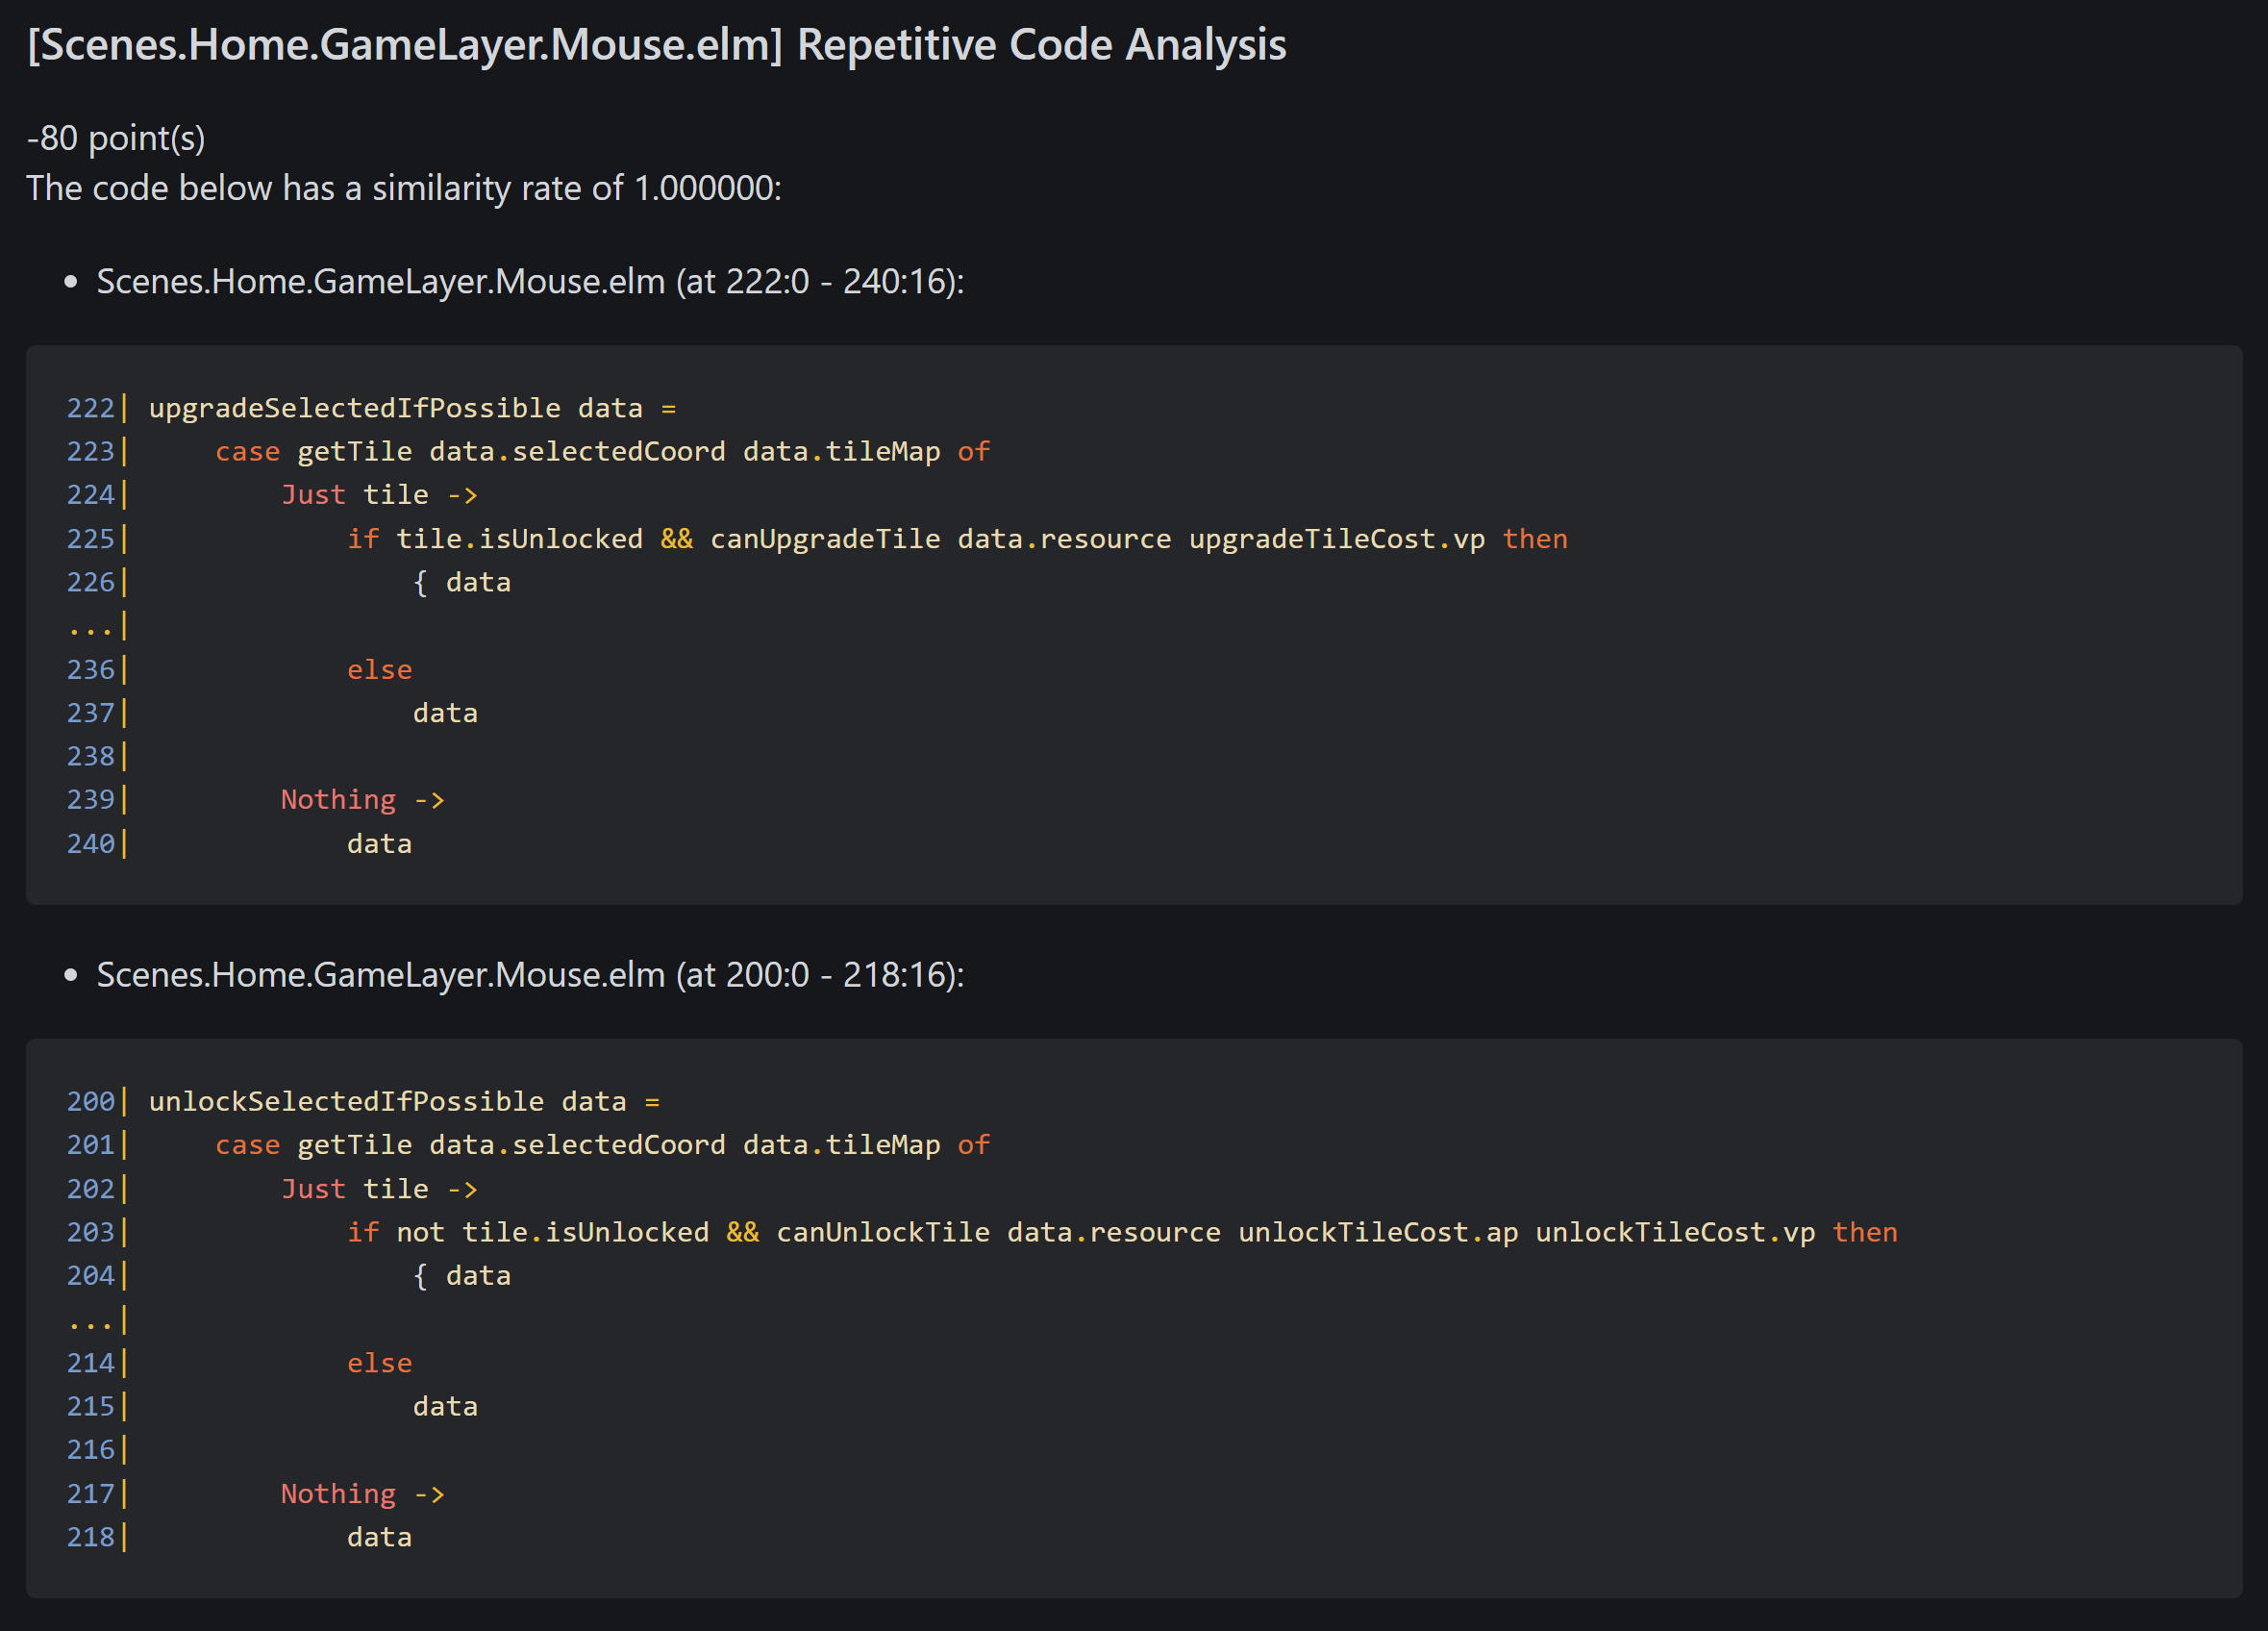
\includegraphics[width=\columnwidth]{repeat2}
\end{frame}

\begin{frame}{Discussion on Code Quality}
	\em Why duplicated code is considered bad? \em
	\bigskip\raggedright
	\pause
	\begin{itemize}
		\item \textbf{Maintenance}: When the same logic is repeated in multiple places, any changes or bug fixes need to be made in every instance, which increases the risk of introducing inconsistencies or errors. It becomes time-consuming and error-prone to keep the duplicated sections in sync.
		\item \textbf{Code readability and understandability}: It leads to unnecessary code bloat, increases complexity, and reduces the overall clarity of the code. Developers who work on the codebase may have to spend more time deciphering duplicated sections, which slows down the development process.
	\end{itemize}
\end{frame}

\begin{frame}{Design Patterns in FP}
	Solution: Use \textbf{design patterns}!
	\begin{definition}
		\textbf{Design patterns} are mainly used to improve code safety and maintainability, including reducing duplicated code.
	\end{definition}
\end{frame}

\section{Example: Error Handling}

\begin{frame}[fragile]{Calculation with Error Handling}
	Two operations with basic error raising:
	\begin{codetbox}{elm}
minusOne : Int -> Maybe Int
minusOne x =
    -- require x >= 0
    if x >= 0 then
        Just (x - 1)
    else
        Nothing

half : Int -> Maybe Int
half x =
    -- require x is even
    if modBy 2 x == 0 then
        Just (x // 2)
    else
        Nothing
	\end{codetbox}

\end{frame}

\begin{frame}[fragile]{Calculation with Error Handling}
	Now see this call function:
	\begin{codetbox}{elm}
call1 : Int -> Maybe Int
call1 x =
    case half x of
        Just h ->
            case minusOne h of
                Just m ->
                    Just m

                Nothing ->
                    Nothing

        Nothing ->
            Nothing
	\end{codetbox}
	Can you comment on the quality of this function?

	\pause
	\em How to avoid the nested pattern matching? \em
\end{frame}

\begin{frame}[fragile]{Maybe and Then \& Ap Operators}
	Read \href{https://package.elm-lang.org/packages/elm/core/latest/Maybe#andThen}{Maybe.andThen}: how does it help with improving the code quality?
	\begin{codetbox}{elm}
andThen : (a -> Maybe b) -> Maybe a -> Maybe b
andThen callback maybe =
  case maybe of
    Just value ->
      callback value

    Nothing ->
      Nothing
	\end{codetbox}
	\begin{codetbox}{elm}
call1 : Int -> Maybe Int
call1 x =
    half x
        |> Maybe.andThen minusOne
-- The same as `Maybe.andThen minusOne (half x)`
	\end{codetbox}
\end{frame}

\begin{frame}[fragile]{More Calculations}
	How to get $x/2-3$?
	\pause
	\begin{codetbox}{elm}
call2 : Int -> Maybe Int
call2 x =
    half x
        |> Maybe.andThen minusOne
        |> Maybe.andThen minusOne
        |> Maybe.andThen minusOne
	\end{codetbox}
\end{frame}

\begin{frame}[fragile]{Bind Operator}
	Alternatively, we introduce the \textbf{bind} operator:
	\begin{codetbox}{elm}
bind : Maybe a -> (a -> Maybe b) -> Maybe b
bind x f =
    Maybe.andThen f x
-- Reverse the order of arguments     
	\end{codetbox}
	It only \textbf{reverses the order} of arguments of {\tt Maybe.andThen}.
	\pause
	\begin{codetbox}{elm}
call2alt : Int -> Maybe Int
call2alt x =
    bind (half x) <| \a ->
    bind (minusOne a) <| \b ->
    bind (minusOne b) <| \c ->
    minusOne c  
	\end{codetbox}
	\pause
	\em What's the data type of {\tt a}, {\tt b} and {\tt c}? \em
\end{frame}

\section{Example: Logger}

\begin{frame}[fragile]{Logging Calculations}
	Let's start with more calculations:
	\begin{codetbox}{elm}
square : Int -> Int
square x =
    x * x

addOne : Int -> Int
addOne x =
    x + 1

call3 : Int
call3 =
    3 |> square |> addOne |> square
	\end{codetbox}
	\pause
	\em How to trace the calculation process, e.g. {\tt ( 1, "Square 1" )}? \em
\end{frame}

\begin{frame}[fragile]{Logging Calculations}
	\begin{codetbox}{elm}
type alias IntWithLogs =
    ( Int, List String )

square : IntWithLogs -> IntWithLogs
square ( x, o ) =
    ( x * x, o ++ [ "Square " ++ fromInt x ] )

addOne : IntWithLogs -> IntWithLogs
addOne ( x, o ) =
    ( x + 1, o ++ [ "AddOne " ++ fromInt x ] )

call3 : IntWithLogs
call3 =
    ( 3, [] ) |> square |> addOne |> square
	\end{codetbox}
	\pause
	Issue 1: We need to manually create the initial {\tt IntWithLogs}, which can cause
	duplicated code.

\end{frame}

\begin{frame}[fragile]{Wrapping function}
	We need a \textbf{wrapping function} that wraps the integer to {\tt IntWithLogs}:
	\begin{codetbox}{elm}
wrapInt : Int -> IntWithLogs
wrapInt x =
  ( x, [] )
	\end{codetbox}
	New {\tt call3}:
	\begin{codetbox}{elm}
call3 : IntWithLogs
call3 =
  3 |> wrapInt |> square |> addOne |> square
	\end{codetbox}
	\pause
	Issue 2: The concatenation of list is duplicated in both {\tt square} and {\tt addOne} functions.
\end{frame}

\begin{frame}[fragile]{Concatention}
	We want to move the logic of concatenation to a new function so that we can reuse it.
	\begin{codetbox}{elm}
runWithLogs : IntWithLogs -> (Int -> IntWithLogs) -> IntWithLogs
runWithLogs ( x, o ) transform =
    let
        ( x_, o_ ) =
            transform x
    in
    ( x_, o ++ o_ )
	\end{codetbox}
	Here {\tt transform} can be fed with {\tt square} or {\tt addOne}.
\end{frame}

\begin{frame}[fragile]{Exapmle 2}
	Change the remaining part of the code accordingly:
	\begin{codetbox}{elm}
square : Int -> IntWithLogs
square x =
    ( x * x, [ "Square " ++ fromInt x ] )

addOne : Int -> IntWithLogs
addOne x =
    ( x + 1, [ "AddOne " ++ fromInt x ] )

call3 : IntWithLogs
call3 =
  let
    x = runWithLogs (wrapInt 3) square
    y = runWithLogs x addOne
  in
    runWithLogs y square
	\end{codetbox}

\end{frame}

\begin{frame}[fragile]{Monadic style}
	Change {\tt call3} for better readability:
	\begin{codetbox}{elm}
call3 : IntWithLogs
call3 =
    runWithLogs (square 3) <| \x ->
    runWithLogs (addOne x) <| \y ->
    square y
	\end{codetbox}
	\pause
	This is called the \textit{Monadic} style.

	\pause
	An important difference between the monadic style and the original style
	is that {\tt x} and {\tt y} are of type {\tt Int} in the former while {\tt IntWithLogs} in the
	latter. The monadic style allows the direct use of previous result in the
	subsequent chaining, and is easier to modify.

	\pause
	It is easy to extend the functionalities in this design pattern. You can add
	calculating functions that only focuses on calculation. All things related
	to logging are hidden by the {\tt runWithLogs} function.
\end{frame}

\begin{frame}{Exercise}
	\begin{itemize}
		\item Add new functions {\tt annihilate} (turn a nonzero interger to 0, return {\tt Nothing} when input is 0) to Example 1, and {\tt multiple} to Example 2. Afterwards, modify the call functions to test them.
		\item Find the similarities between the two examples.
	\end{itemize}
\end{frame}


\begin{frame}{Monad}
	Okay, I noticed that there are some similarities between the {\tt Maybe} and
		{\tt IntWithLogs}. So what are they on earth?

	\medskip\pause

	They are called \textbf{Monads}. It sounds spooky but once you understand it,
	it is very simple and useful. In FP, you can think of monad as a strategy
	for combining computations into more complex computations.

	\medskip\pause



	In the above 2 examples we covered two monads: the \textbf{Maybe} monad and the \textbf{Writer} monad.
\end{frame}

\section{Monad}

\begin{frame}{What is a monad?}
	A monad contains three things:

	\begin{itemize}
		\item \textbf{A type constructor} {\tt M} that takes a type {\tt a} and returns a new type {\tt M~a}. You can think of this as a \textbf{container} of type {\tt a}, e.g. {\tt Maybe}.
		\item \textbf{A function} {\tt return: a -> M~a}, used to wrap a value of type {\tt a} into the container {\tt M}.
		\item \textbf{A function} {\tt bind: M~a~->~(a~->~M~b)~->~M~b}\footnote{An alternative equivalent definition is {\tt join: M (M a) -> M a}.}, used to bind the result of a computation to some symbol you can use in the second argument function.
	\end{itemize}

	\medskip\pause

	\em Identify the three components of the monads in the examples above. \em
	\medskip\pause

	\em A monad is just a monoid in the category of endofunctors. \em -- James Iry

\end{frame}

\begin{frame}[fragile]{Try playing with Monad in Elm}
	Elm doesn't support \textit{Higher Kinded Types} (for example, {\tt template} in C++), so we cannot define a general monad signature/type in Elm.
	\medskip\pause

	However, we can still write them by defining those functions separately for each monad.
	\medskip\pause

	\textbf{Exercise: }

	List is also a Monad! Try find out the constuctor, {\tt return} and {\tt bind} functions for it. Then, write a function that returns a list of all possible results of multiplying two integers in two respective lists.

	\textbf{Hint}: The {\tt bind} function is applied to all possible values in the input list and the resulting lists are concatenated to produce a list of all possible results.
\end{frame}
\begin{frame}[fragile]{Package for Common Mondas}
	\href{https://package.elm-lang.org/packages/linsyking/elm-monad/latest/}{elm-monad} is an elm package that exposes several useful monads for Elm.

	Try installing this package in a project:
	\begin{codetbox}{bash}
elm install linsyking/elm-monad
	\end{codetbox}
	Then import related modules:
	\begin{codetbox}{elm}
import Monad.Writer exposing (..)
	\end{codetbox}
	If you want to use multiple monads in a module, you need to \textbf{rename} the module because their functions have conflicts.
	
	\medskip\pause
	\em Rewrite the previous exercise with {\tt Monad.List}. \em
\end{frame}
\begin{frame}{Mindsets}

	\begin{itemize}
\item Monad is not FP only. It is a general design pattern in programming.
\item You can think of Monad as an interface or abstract class and the
return and bind functions are the abstract methods. Different monad
instances have different implementations of those functions.
\item One container type may have different return and bind functions.
So there might be different monads for the same container type.
However, there is usually only one monad for a container type and
those functions are determined by the container itself.
\item You may have additional helper functions for a monad.
\end{itemize}

\end{frame}
\begin{framek}[Conclusion]
	Today you earned a new design pattern called Monad. Hopefully it doesn't sound any more mysterious and difficult for you.
	\medskip

	If you find monad helpful and want to learn more about monad, you can start by looking at the {\tt State} monad, which is a generalization of the {\tt Writer} monad and is helpful for writing random generators. You may also refer to these website:
	\begin{itemize}
		\item Youtube. \href{https://www.youtube.com/watch?v=C2w45qRc3aU}{The Absolute Best Intro to Monads For Software Engineers}
		\item Haskell Wiki. \href{https://wiki.haskell.org/All_About_Monads}{All About Monads}
		\item Wikipedia. \href{https://en.wikipedia.org/wiki/Monad_(functional_programming)}{Monad (functional programming)}
	\end{itemize}
\end{framek}


\end{document}
